%!TEX root = ../thesis.tex
%*******************************************************************************
%****************************** Chapter 5 **************************************
%*******************************************************************************

\chapter{SYSTEM DESIGN AND IMPLEMENTATION}
\label{chap:system}

\ifpdf
    \graphicspath{{Chapter5/Figs/Raster/}{Chapter5/Figs/PDF/}{Chapter5/Figs/}}
\else
    \graphicspath{{Chapter5/Figs/Vector/}{Chapter5/Figs/}}
\fi

Chapter~\ref{chap:methods} defined the method. This chapter describes the system that turns
the method into a working application: a web prototype that answers a Vietnamese question
about an image and shows the text it read as evidence. Section~\ref{sec:sd-req} states the
requirements. Section~\ref{sec:sd-arch} presents the architecture and how the adapted model
is integrated with OCR and the interface, and Section~\ref{sec:sd-flow} follows the data
through the system. Section~\ref{sec:sd-impl} describes the implementation,
Section~\ref{sec:met-proto} the user interface and the inference rules specific to the
prototype, Section~\ref{sec:sd-deploy} the deployment, Section~\ref{sec:res-proto} the
verification, and Section~\ref{sec:sd-scale} scalability and maintenance. The commands needed
to rebuild the system are listed in Appendix~\ref{appendix:repro}.

%********************************** Section 5.1 ********************************
\section{Requirements}
\label{sec:sd-req}

The project proposal asks for a web prototype that accepts a Vietnamese image and question,
generates a natural-language answer and shows the model's confidence and, where relevant,
the extracted OCR text. Table~\ref{tab:sd-req} turns this into functional (F) and
non-functional (N) requirements and shows where each one is met.

\begin{table}[htbp]
\caption{Requirements of the prototype}
\label{tab:sd-req}
\centering
\small
\begin{tabular}{p{0.06\textwidth}p{0.40\textwidth}p{0.44\textwidth}}
\toprule
\raggedright \textbf{ID} & \raggedright \textbf{Requirement} & \raggedright \textbf{How it is met} \tabularnewline
\midrule
\raggedright F1 & \raggedright Upload an image (file or clipboard) and type a Vietnamese question of up to 300 characters & \raggedright Gradio web interface (Section~\ref{sec:met-proto}) \tabularnewline
\raggedright F2 & \raggedright Return a short Vietnamese answer & \raggedright Qwen2.5-VL-3B-Instruct with the SH adapter, greedy decoding (Section~\ref{sec:sd-arch}) \tabularnewline
\raggedright F3 & \raggedright Show the model's confidence & \raggedright Confidence level High, Medium or Low (Section~\ref{sec:met-proto}) \tabularnewline
\raggedright F4 & \raggedright Show the OCR text used as evidence & \raggedright Numbered text boxes on the image and the list of OCR lines (Section~\ref{sec:met-proto}) \tabularnewline
\raggedright N1 & \raggedright Fidelity: the same answers as the evaluated system & \raggedright Inference code shared with the evaluation; rules R-PAR, R-OCR and R-LIVE (Section~\ref{sec:res-proto}) \tabularnewline
\raggedright N2 & \raggedright Efficiency: one Colab GPU, or a laptop GPU with 4~GB & \raggedright Base model in 4 bits, adapter of about 30~MB, OCR in its own process (Section~\ref{sec:sd-deploy}) \tabularnewline
\raggedright N3 & \raggedright Privacy: users' images and questions are not stored & \raggedright Only processing measurements are logged (Section~\ref{sec:sd-flow}) \tabularnewline
\raggedright N4 & \raggedright Reproducibility: every component can be checked & \raggedright Versions, SHA-256 hashes and run signatures (Section~\ref{sec:sd-scale}) \tabularnewline
\bottomrule
\end{tabular}
\end{table}

%********************************** Section 5.2 ********************************
\section{Architecture and AI model integration}
\label{sec:sd-arch}

Figure~\ref{fig:sd-arch} shows the components of the prototype. The system runs as two
processes on one machine.

\begin{figure}[htbp]
\centering
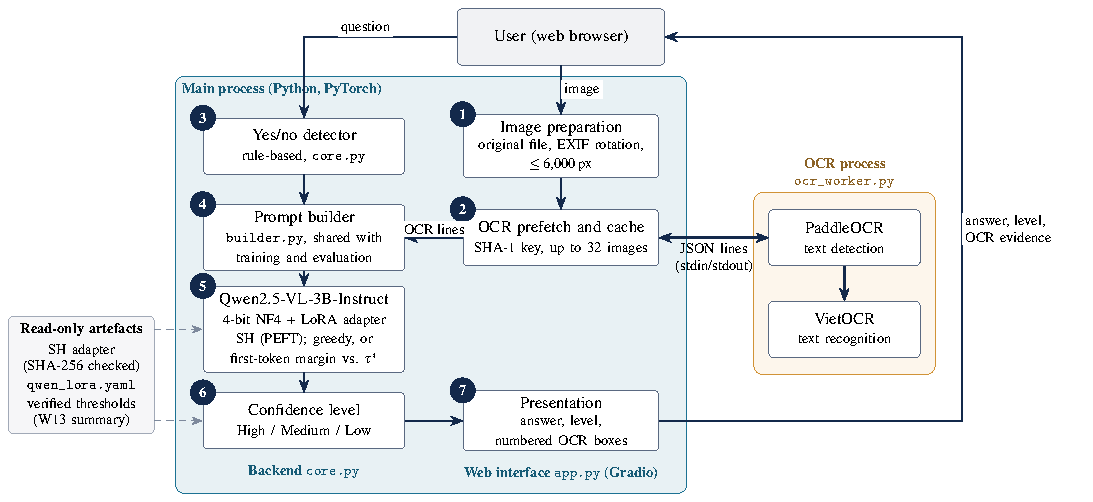
\includegraphics[width=\linewidth]{sd_architecture.pdf}
\caption[Architecture of the prototype]{Architecture of the prototype. The numbers follow
the steps of the online data flow in Section~\ref{sec:sd-flow}. The main process never loads
PaddleOCR; the two processes exchange one JSON message per line.}
\label{fig:sd-arch}
\end{figure}

\paragraph{Main process.} The main process hosts the web interface and the model. The
interface (\path{src/prototype/app.py}) is a Gradio~\cite{abid2019gradio} application that
receives the image and the question and renders the result. Behind it, a \texttt{Backend}
object (\path{src/prototype/core.py}) loads Qwen2.5-VL-3B-Instruct once, in 4-bit NF4 and
with the same configuration file as the evaluation (\path{configs/qwen_lora.yaml}), attaches
the SH adapter with PEFT, and then answers any number of questions. The model is therefore
integrated as a library inside the backend rather than as a separate service: the interface
calls one method, \texttt{Backend.ask(image, question, OCR lines)}, and receives a record
with the answer, the answer mode (open or yes/no), the confidence and its level, the OCR
lines used and the time spent in each step.

\paragraph{OCR process.} OCR runs in a child process (\path{src/prototype/ocr_worker.py}) that
keeps PaddleOCR (text detection) and VietOCR (text recognition) loaded. The two processes
exchange one JSON message per line over the standard input and output: the main process sends
an identifier and an image path, and the worker returns the text lines with their boxes and
confidences, or an error. There are two reasons for this separation. First, the GPU build of
PaddleOCR ships its own CUDA libraries, which conflict with PyTorch when both are loaded in
one process (Table~\ref{tab:pm-risks}). Second, the worker must use exactly the engine that
built the OCR cache of the evaluation: at start-up it reports the PaddleOCR version, the
detection and recognition models, the VietOCR configuration and the language, and the
prototype refuses to start if any of them differs from the cache.

\paragraph{Code shared with the evaluation.} The prototype does not re-implement the method.
It calls the prompt builder used for training and evaluation (\path{src/prompting/builder.py}),
the model loader of the evaluation (\path{src/eval/run_baseline.py}) and the function that turns
OCR lines into the OCR line of the prompt (\path{src/data/ocr.py}). This is what makes
requirement N1 testable.

\paragraph{Verified settings.} The thresholds of the confidence levels and of the yes/no
decision are not typed by hand. The interface reads them from the summary file of the
verification run (\path{experiments/W13_prototype_check_L4_seed42/prototype_check_summary.json})
and checks that the value of $\tau^*$ in that file equals the constant in \path{core.py}. The
real model is loaded only if the rules R-PAR, R-CONF and R-YB-det recorded in that file have
passed; otherwise the application stops with an error.

%********************************** Section 5.3 ********************************
\section{Data flow and processing}
\label{sec:sd-flow}

The system has two data flows. The \emph{offline flow} is the research pipeline of
Chapter~\ref{chap:methods} (Figure~\ref{fig:met-pipeline}): data preparation, the OCR cache,
training and evaluation. It produces the adapters and the list of official models in
\path{configs/official_models.json}. The \emph{online flow} answers one question in the
prototype and reuses the artefacts of the offline flow. It has seven steps
(Figure~\ref{fig:sd-arch}):

\begin{enumerate}
  \item \textbf{Image preparation.} The uploaded image is used as the original file, exactly
  as in the evaluation. Only an image with an EXIF rotation flag or with a side longer than
  6,000 pixels is rotated or reduced and saved losslessly as PNG. Formats that cannot be read,
  such as HEIC, are rejected with a message.
  \item \textbf{OCR in the background.} As soon as the image is uploaded, an OCR job starts in
  the worker. Its result is kept in an in-memory cache of up to 32 images, keyed by the SHA-1
  hash of the prepared image, so further questions about the same image do not run OCR again.
  \item \textbf{Question routing.} A rule-based detector decides whether the question is a
  yes/no question (Section~\ref{sec:met-proto}).
  \item \textbf{Prompt.} The OCR lines, in reading order and cut to 600 characters, form the
  OCR line of the prompt with the template chosen in W08 (Section~\ref{sec:met-prompt}); the
  prompt is built by the shared prompt builder.
  \item \textbf{Generation.} An open question is answered by greedy decoding with at most 32
  new tokens. A yes/no question receives the answering instruction of POPE-vi and is decided
  by the first-token margin against $\tau^*$.
  \item \textbf{Confidence.} The confidence is mapped to a level with the verified thresholds.
  \item \textbf{Presentation.} The interface shows the answer, the level, the OCR lines and an
  image with the numbered text boxes. Only this display copy is reduced, to at most 1,280
  pixels per side; the model and OCR always use the full-resolution image.
\end{enumerate}

Nothing is kept after the session: images, questions and answers are not saved, and the
optional log records only measurements (processing times, the confidence level, the number
of OCR lines and the image size).

%********************************** Section 5.4 ********************************
\section{Implementation}
\label{sec:sd-impl}

\paragraph{Technology.} The system is written in Python. Table~\ref{tab:sd-stack} lists the
main libraries and their roles; the exact versions are pinned in \path{requirements-colab.txt}
(Section~\ref{sec:met-setup}).

\begin{table}[htbp]
\caption{Main technologies of the system}
\label{tab:sd-stack}
\centering
\small
\begin{tabular}{p{0.20\textwidth}p{0.36\textwidth}p{0.34\textwidth}}
\toprule
\raggedright \textbf{Layer} & \raggedright \textbf{Libraries and tools} & \raggedright \textbf{Role} \tabularnewline
\midrule
\raggedright Model and adaptation & \raggedright PyTorch, Transformers, PEFT, bitsandbytes, Accelerate, qwen-vl-utils & \raggedright Load Qwen2.5-VL-3B-Instruct in 4 bits, train and attach LoRA adapters, turn images into image tokens \tabularnewline
\raggedright OCR & \raggedright PaddleOCR (detection), VietOCR (recognition) & \raggedright Read Vietnamese text in images \tabularnewline
\raggedright Evaluation and analysis & \raggedright NumPy, pandas, pyvi, openpyxl & \raggedright Metrics, paired tests, error analysis, annotation sheets \tabularnewline
\raggedright Interface & \raggedright Gradio & \raggedright Web application \tabularnewline
\raggedright Execution & \raggedright Google Colab (L4, T4); Windows laptop; Git and Google Drive & \raggedright Training, evaluation and demonstration; code and artefact storage \tabularnewline
\bottomrule
\end{tabular}
\end{table}

\paragraph{Source-code organisation.} Table~\ref{tab:sd-code} maps the directories of the
repository to the parts of the system. The repository contains 49 Python modules, 30 Colab
notebooks and the logs of 142 runs.

\begin{table}[htbp]
\caption{Organisation of the source code}
\label{tab:sd-code}
\centering
\small
\begin{tabular}{p{0.20\textwidth}p{0.42\textwidth}p{0.28\textwidth}}
\toprule
\raggedright \textbf{Directory} & \raggedright \textbf{Main modules} & \raggedright \textbf{Part of the system} \tabularnewline
\midrule
\raggedright \path{src/data/} & \raggedright \path{prepare_vivqa.py}, \path{prepare_vitextvqa.py}, \path{make_train_subset.py}, \path{check_split_overlap.py}, \path{ocr.py}, \path{exif_audit.py} & \raggedright Data preparation, splits, OCR cache \tabularnewline
\raggedright \path{src/prompting/} & \raggedright \path{builder.py} & \raggedright One prompt builder for training, evaluation and the prototype \tabularnewline
\raggedright \path{src/models/}, \path{src/adaptation/} & \raggedright \path{vlm_loader.py}, \path{train_qlora.py}, \path{lora_targets.py} & \raggedright Model loading, QLoRA training, choice of LoRA layers \tabularnewline
\raggedright \path{src/eval/} & \raggedright \path{run_baseline.py}, \path{metrics.py}, \path{full_eval_table.py}, \path{pope_vi.py}, \path{error_analysis.py}, \path{yesno_calib.py}, \path{repro_manifest.py} & \raggedright Inference, metrics, analyses, list of official models \tabularnewline
\raggedright \path{src/prototype/} & \raggedright \path{core.py}, \path{app.py}, \path{ocr_worker.py}, \path{infer.py} & \raggedright Backend, web interface, OCR process, command-line inference \tabularnewline
\raggedright \path{configs/} & \raggedright \path{qwen_lora.yaml}, \path{official_models.json} & \raggedright Shared configuration; official models with hashes \tabularnewline
\raggedright \path{notebooks/} & \raggedright 30 notebooks, numbered 00--29 & \raggedright Colab entry points, one per experiment \tabularnewline
\raggedright \path{experiments/} & \raggedright One directory per run & \raggedright Logs, predictions, run signatures \tabularnewline
\bottomrule
\end{tabular}
\end{table}

\paragraph{Engineering practices.} Three practices keep the implementation consistent with the
numbers in the thesis. First, the main modules have a \texttt{-{}-selftest} mode that runs on
the CPU on both Windows and Linux, and the interface and the command-line tool also have a
\texttt{-{}-mock} mode with a fake backend, so the interface can be developed without a GPU.
Second, the constants that change the answers (the core version, the yes/no detector version
and $\tau^*$) are fixed in the code and recorded in the run signature; changing one of them
means a new run. Third, the training and evaluation scripts refuse to resume a run whose
configuration differs from its signature (Section~\ref{sec:met-setup}).

%********************************** Section 5.5 ********************************
\section{User interface and prototype-specific rules}
\label{sec:met-proto}

Figure~\ref{fig:sd-ui} shows the interface; its labels are in Vietnamese because the system is
intended for Vietnamese users. The left column holds the image (uploaded from a file or pasted
from the clipboard), the question box and the buttons \emph{Answer} (``\vi{Trả lời}'') and
\emph{Clear} (``\vi{Xoá}''). The right column shows the answer with its confidence level and
question mode, a note saying whether the answer matches a line of OCR text, and three
collapsible panels: the OCR evidence (the image with the text boxes numbered in reading order,
the matching line in green, and the list of lines), technical details (mode, timing, image
size, OCR settings and the prompt sent to the model) and an explanation of the confidence
level. A notice at the bottom states that the system is a research prototype that can give
wrong or hallucinated answers, must not be used for important decisions, and does not keep
the user's images or questions.

\begin{figure}[htbp]
\centering
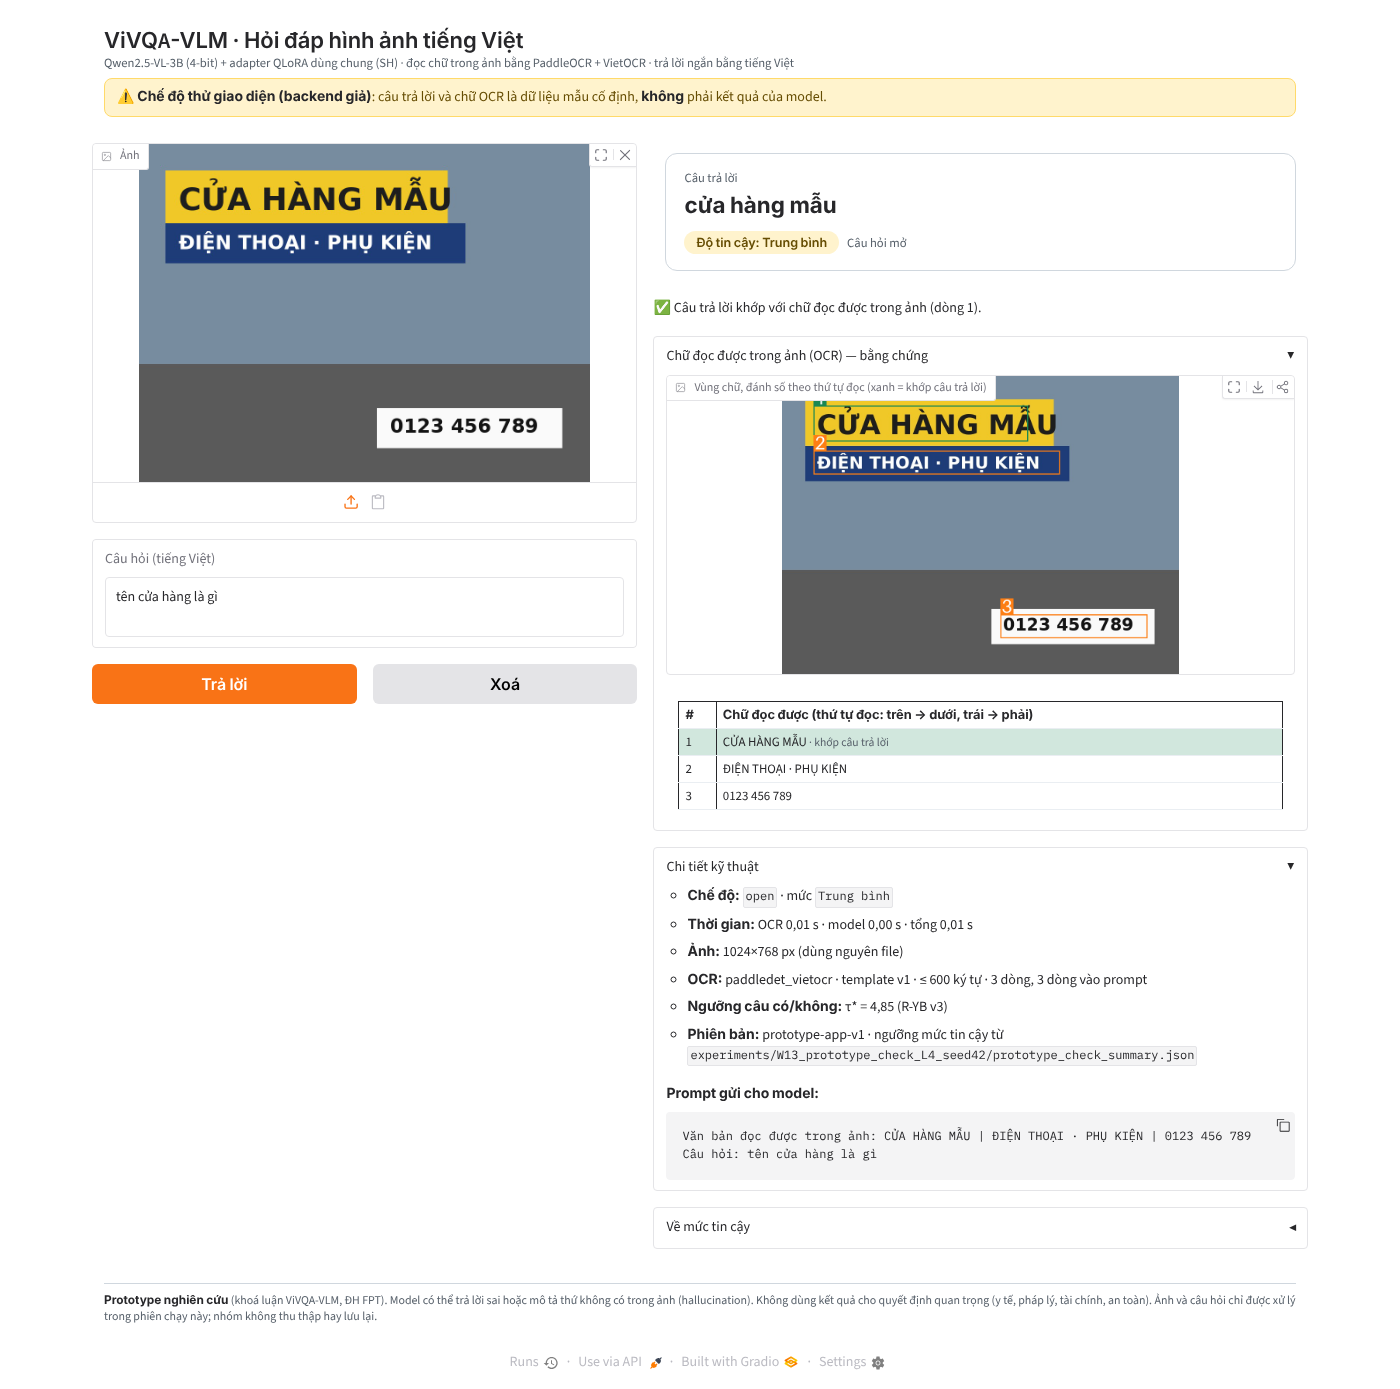
\includegraphics[width=\linewidth,height=0.62\textheight,keepaspectratio]{sd_interface.png}
\caption[The web interface of the prototype]{The web interface of the prototype (labels in
Vietnamese). The screenshot was taken in the interface-test mode with a mock backend: the
image is a synthetic sample and the answer is not a model output.}
\label{fig:sd-ui}
\end{figure}

The prototype follows three design principles:

\begin{enumerate}
  \item \textbf{The same inference path as the evaluation.} The prototype calls exactly
  the prompt-building function, the adapter and the decoding (greedy, at most 32 tokens)
  of the evaluation pipeline. This is checked with the matching rule in
  Section~\ref{sec:res-proto}.
  \item \textbf{Answers with evidence.} Because the model uses OCR, the interface shows
  the OCR text so that users can check the answer themselves. OCR runs in a separate
  process and reads the original image (at most 6,000 pixels per side) rotated according
  to the EXIF flag.
  \item \textbf{One adapter for every question.} The prototype uses the SH adapter,
  trained on both ViVQA and ViTextVQA, so it does not need to guess in advance which kind
  of question the user will ask.
\end{enumerate}

\paragraph{Confidence.} For open questions, the confidence is the $\exp$ of the mean log
probability of the answer tokens. Because this confidence is not well calibrated
(ECE~\cite{guo2017calibration} of 0.198), the interface shows only High, Medium or Low
instead of a percentage.

\paragraph{Yes/no questions.} A rule-based detector flags yes/no questions (ending in
``\vi{không}'', ``\vi{chưa}'', ``\vi{phải không}''\ldots{} and containing no question
word). For these questions, the decision is based on the margin
$m = s_{\text{yes}} - s_{\text{no}}$ between the largest log probability of a first token
on the ``yes'' side and on the ``no'' side: the answer is ``yes'' when $m > \tau^*$. The
threshold $\tau^* = 4.85$ is chosen on a separate calibration set (ViVQA test images not
seen in training and not part of POPE-vi) by maximising the balanced accuracy, in order to
correct SH's ``yes'' bias (Section~\ref{sec:dis-halluc}) without retraining. Other
questions go through the greedy path as in the evaluation.

%********************************** Section 5.6 ********************************
\section{Deployment}
\label{sec:sd-deploy}

The same code is deployed in two configurations (Table~\ref{tab:sd-deploy}): on Google Colab
for development, verification and sharing, and offline on a laptop for the live
demonstration at the defence.

\begin{table}[htbp]
\caption{Deployment configurations}
\label{tab:sd-deploy}
\centering
\small
\begin{tabular}{p{0.20\textwidth}p{0.34\textwidth}p{0.36\textwidth}}
\toprule
\raggedright \textbf{Item} & \raggedright \textbf{Cloud (Google Colab)} & \raggedright \textbf{Laptop (offline)} \tabularnewline
\midrule
\raggedright Hardware & \raggedright NVIDIA L4, 24~GB & \raggedright NVIDIA RTX 3050 Ti, 4~GB; 16~GB RAM; Windows 11 \tabularnewline
\raggedright Placement & \raggedright Model, adapter and OCR on the GPU (OCR falls back to the CPU if the GPU build of PaddleOCR cannot be installed) & \raggedright 4-bit model and adapter on the GPU; OCR on the CPU \tabularnewline
\raggedright Start & \raggedright Notebook \path{28_prototype_v2_live_demo_sh_qwen25vl.ipynb} & \raggedright One click on \path{demo.cmd} (script \path{run_local_windows.ps1}) \tabularnewline
\raggedright Access & \raggedright Public link \path{*.gradio.live} & \raggedright \path{http://127.0.0.1:7860}, no Internet connection needed \tabularnewline
\raggedright Start-up time & \raggedright About 60~s (measured in W13) & \raggedright About 27~s (parallel start), 47.9~s (sequential start) \tabularnewline
\raggedright Time per question & \raggedright Median 1.00~s, 95th percentile 3.58~s & \raggedright Median 0.93~s once OCR has finished in the background; 7.39~s right after the upload \tabularnewline
\raggedright GPU memory & \raggedright 4.78~GB in total & \raggedright At most 2.40~GB \tabularnewline
\bottomrule
\end{tabular}
\end{table}

\paragraph{Deployment procedure.} (1) Clone the repository and install the pinned libraries:
\path{requirements-colab.txt} on Colab, a dedicated Python environment on the laptop.
(2) Obtain the SH adapter and check its SHA-256 hash against
\path{configs/official_models.json}; both launchers pass the expected hash to the application
(option \texttt{-{}-expect\_adapter\_sha}), and the command-line tool checks it with the
option \texttt{-{}-official sh}. (3) Start the application: on Colab, run notebook 28, which
re-checks rules R-OCR and R-LIVE before opening the link; on the laptop, run \path{demo.cmd}.
(4) At start-up, the application checks the OCR engine against the cache and loads the
verified settings, and it stops if either check fails. For scripted use without the
interface, \path{src/prototype/infer.py} runs the same path from the command line and writes
one JSON line per question (Appendix~\ref{appendix:repro}).

%********************************** Section 5.7 ********************************
\section{Verification and testing}
\label{sec:res-proto}

Testing works at two levels. At the module level, the self-tests run before every commit
(Section~\ref{sec:sd-impl}). At the system level, the checks below compare the prototype
with the evaluated system.

The prototype must give exactly the same answers as the evaluation pipeline; otherwise the
numbers in the thesis no longer hold for the demo. We set five rules before checking
(Table~\ref{tab:res-proto}); all five pass after fixing the image downscaling threshold in
version 2.

\begin{table}[htbp]
\caption{Prototype verification against pre-set rules}
\label{tab:res-proto}
\centering
\small
\begin{tabular}{p{0.38\textwidth}p{0.16\textwidth}p{0.36\textwidth}}
\toprule
\raggedright \textbf{Rule} & \raggedright \textbf{Result} & \raggedright \textbf{Meaning} \tabularnewline
\midrule
\raggedright R-PAR: backend matches the evaluation pipeline & \raggedright 100\% & \raggedright Same answers as the official evaluation run \tabularnewline
\raggedright R-LIVE: through the interface, live OCR & \raggedright 100\% / 100\% & \raggedright 200 images each for ViVQA / ViTextVQA \tabularnewline
\raggedright R-OCR: OCR through the interface equals direct OCR & \raggedright 100\% / 100\% & \raggedright After raising the image threshold to 6,000 pixels per side \tabularnewline
\raggedright R-CONF: confidence levels are meaningful & \raggedright Pass & \raggedright EM decreases from High to Medium to Low \tabularnewline
\raggedright R-YB: ``yes'' bias corrected & \raggedright Pass & \raggedright $\tau^* = 4.85$; ``yes'' ratio 41--45\% \tabularnewline
\bottomrule
\end{tabular}
\end{table}

On a Colab L4, the median latency is 1.00 second and the 95th percentile 3.58 seconds per
question, with 4.78~GB of VRAM. On 20 photos that we took, the prototype answers 14
questions correctly, including all 5 yes/no questions. The first version failed rule R-OCR
(87.5\% on ViTextVQA) because the interface downscaled images larger than 2,048 pixels
before OCR, while 1,418 ViTextVQA images exceed this threshold; raising the threshold to
6,000 pixels fixed the problem.

We also run the prototype offline on a laptop with an NVIDIA RTX 3050 Ti (4~GB) and 16~GB
of RAM, with the same adapter, prompt and decoding settings. The model uses at most
2.40~GB of VRAM, and system memory use peaks at 13.5 of 15.7~GB during start-up. On the
same 20 photos, the laptop gives exactly the same answers as Colab for all 20 questions.
On five example questions, the median time per question is 0.93 seconds when OCR has
already finished in the background, and 7.39 seconds when the question is asked right after
the upload; the difference is almost entirely OCR on the CPU. The application is ready
about 27 seconds after start-up.

%********************************** Section 5.8 ********************************
\section{Scalability and maintenance}
\label{sec:sd-scale}

\paragraph{Capacity.} The prototype is designed for one user at a time: the Gradio queue
processes one request at a time on one GPU, and the OCR cache holds 32 images. This is
enough for a demonstration and for the verification runs, but not for many simultaneous
users.

\paragraph{Scaling.} Because the model is loaded once and the interface reaches it through a
single method, the system can be scaled without changing the method: several backend
processes, one per GPU, can serve requests behind a load balancer, and several questions can
be batched into one forward pass. On the laptop, OCR on the CPU is the slowest step; running
OCR on a GPU, or computing it in advance as the evaluation does, removes most of the waiting
time. These options were not implemented or measured in this thesis.

\paragraph{Extending the system.} The base model is shared, and the task-specific knowledge
sits in a small adapter of about 30~MB. Adding a dataset or a task therefore means building
its OCR cache with the same engine, training a new adapter with
\path{src/adaptation/train_qlora.py}, evaluating it with \path{src/eval/run_baseline.py} and
registering it in \path{configs/official_models.json}; the interface and the backend do not
change.

\paragraph{Version management and maintenance.} The source code is versioned with Git, the
base model is pinned to a revision on Hugging Face, the adapters, the OCR cache and the data
files are identified by SHA-256 hashes, and the list of official models is regenerated from
the logs (\texttt{python -m src.eval.repro\_manifest -{}-build}) instead of being edited by
hand. The components that affect the answers carry version names in the code, for example
\texttt{prototype-core-v1}, \texttt{yesno-detector-v1}, \texttt{ocr-worker-v1} and
\texttt{prototype-app-v2.2}. The main maintenance risk is change in external libraries and
platforms: library versions are pinned, a newer default PyTorch on Colab must be replaced by
the version recorded in the logs, and an OCR engine that differs from the cache is refused at
start-up (Appendix~\ref{appendix:repro}).
